% ==========================================================================
% INFO 4617 Web Data Science -- Week 11: Government Data APIs (Chapter 11)
% Build:  latexmk -pdf week-11.tex   (from this folder; no env vars needed)
% (or run `make` from the slides/ directory to build every deck)
% ==========================================================================
\documentclass[9pt,aspectratio=169]{beamer}
% Resolve the shared theme/preamble in ../common/ when compiling this
% file directly from its own folder (no TEXINPUTS needed).
\makeatletter\def\input@path{{../common/}}\makeatother
\input{preamble}

\title[Week 11 · Government APIs]{{\Huge Government Data APIs}}
\subtitle{Week 11 · APIs module · Textbook Chapter 11}
\author[Keegan]{\textbf{Brian C. Keegan, Ph.D.} \\ Associate Professor, Department of Information Science \\ University of Colorado Boulder}
\date{October 26, 28 \& 30, 2026}

\begin{document}

\maketitle

% -------------------------------------------------------------------------
\begin{frame}{This week at a glance}
    \begin{columns}[T]
        \begin{column}{0.6\textwidth}
            Three public APIs, each showing one idea that holds for every API. This week, every class is live coding, from one lab notebook in three parts.

            \bigskip

            \dayband{Monday}{Lab, part 1: the Census}
            \begin{itemize}\small
                \item Keys, and \textit{what can I ask for?} --- the variable and geography catalogs
            \end{itemize}

            \medskip

            \dayband{Wednesday}{Lab, part 2: more of the Census, then FRED}
            \begin{itemize}\small
                \item Margins of error and missing estimates; then \textit{let the server compute}
            \end{itemize}

            \medskip

            \dayband{Friday}{Lab, part 3: more of FRED, then the EIA}
            \begin{itemize}\small
                \item \textit{Let the server filter}; then textbook revisions
            \end{itemize}
        \end{column}
        \begin{column}{0.35\textwidth}
            \textbf{The lab}\\[2pt]
            {\footnotesize \texttt{labs/week-11/lab-11.ipynb} in the course repository. Each part is added before its day.\par}
            \medskip
            \begin{alertblock}{Three keys, as environment variables}
                \footnotesize \texttt{CENSUS\_KEY} Monday and Wednesday; \texttt{FRED\_KEY} Wednesday and Friday; \texttt{EIA\_KEY} Friday. Links are in the Canvas announcement and the lab's first cell.
            \end{alertblock}
            \textbf{Due Sunday, Nov 1}\\[2pt]
            {\footnotesize Chapter 11's \textbf{Recommended Exercises}, from its companion notebook. Graded on good-faith attempt to complete rather than getting everything working.\par}
            \medskip
        \end{column}
    \end{columns}
\end{frame}

% =========================================================================
\section{Monday · Live-Coding Lab}
% =========================================================================

\begin{frame}{This week, every class is live coding}
    \begin{columns}[T]
        \begin{column}{0.56\textwidth}
            \dayband{Find it}{\texttt{labs/} in the course repository}
            \begin{enumerate}\small
                \item Open the \href{https://github.com/cuinfoscience/INFO4617-Fall2026/tree/main/labs}{\textbf{labs} folder} of \texttt{cuinfoscience/INFO4617-Fall2026} on GitHub
                \item Open \texttt{week-11}, click \texttt{lab-11.ipynb}, then \textbf{Download raw file}
                \item Open it in JupyterLab in the \texttt{webdata} environment, \textit{after} setting your keys
            \end{enumerate}

            \medskip
            \dayband{Use it}{one part a day}
            \begin{itemize}\small
                \item I write the code on screen, and you write it in your copy
                \item Put \textbf{your} email in the User-Agent in Step 0
                \item Today: Part 1, Steps 0--6, about 50 minutes
                \item Wednesday and Friday: download the new copy and start at that part's setup step
            \end{itemize}
        \end{column}
        \begin{column}{0.4\textwidth}
            \textbf{Solutions}\\[2pt]
            {\footnotesize \texttt{lab-11-key.ipynb}, beside it: every cell filled in and run. Fall behind? Copy the cell from the key and keep going.\par}
            \medskip
            \textbf{Nothing to submit}\\[2pt]
            {\footnotesize The lab is practice. After each step, a \textbf{Discuss} box holds questions we'll talk over before the next.\par}
            \medskip
            \begin{alertblock}{Error flavors}
                \footnotesize A missing key stops Step 0 \textit{on purpose}: set it and run again. A cell that fails with your key set is \textit{broken}: tell me, or open an issue.
            \end{alertblock}
            \textbf{No key yet?}\\[2pt]
            {\footnotesize Follow along: the key shows every output. A Census key works only after you click the link in its email.\par}
            \medskip
        \end{column}
    \end{columns}
\end{frame}

\begin{frame}{Public data by mandate}
    \begin{columns}[T]
        \begin{column}{0.6\textwidth}
            Government APIs exist because of democratic commitments to \textbf{transparency} --- not business strategy:
            \begin{itemize}\small
                \item The \textbf{Census Bureau} is constitutionally mandated to count the population.
                \item The \textbf{Federal Reserve} publishes the economic data it collects; FRED is the St.\ Louis Fed's service for it.
                \item The \textbf{Energy Information Administration} was created in 1977, after the energy crises, to publish independent energy statistics.
                \item The \textbf{Library of Congress} publishes Congress's legislative record at Congress.gov.
            \end{itemize}

            \medskip

            They embody the \textbf{openness} value from Ch.~3, \textit{The Post-API Age}: public data, freely accessible by mandate rather than platform goodwill.
        \end{column}
        \begin{column}{0.35\textwidth}
            \begin{alertblock}{Stable, but less polished}
                \footnotesize Agencies don't pivot business models or get acquired --- so these APIs are unusually \textbf{stable}. The tradeoff: dense docs, cryptic variable names, unhelpful errors. Navigating that \textit{is} the skill.
            \end{alertblock}
        \end{column}
    \end{columns}
\end{frame}

\begin{frame}{Three APIs, three ideas}
    Week 10's Wikipedia taught \textbf{pagination}. Each API this week teaches one more idea you'll meet in every API:

    \medskip
    \begin{center}\small
    \begin{tabular}{@{}lll@{}}
        \toprule
        \textbf{Day} & \textbf{API} & \textbf{The idea} \\
        \midrule
        Monday, Wednesday & Census Bureau & \textbf{Discovery}: ask the API what you can ask for \\
        Wednesday, Friday & FRED & \textbf{Let the server compute}: transforms in the request \\
        Friday & EIA & \textbf{Let the server filter}: facets narrow the data before it's sent \\
        \midrule
        The chapter & Congress.gov & \textbf{Follow the links}: records point to related records \\
        \bottomrule
    \end{tabular}
    \end{center}

    \medskip
    And one idea across all of them: a \textbf{key} says who you are, and it stays out of your notebook.
\end{frame}

\begin{frame}[fragile]{Keys stay out of the notebook}
    \begin{columns}[T]
        \begin{column}{0.56\textwidth}
            A \textbf{key} identifies you, counts your requests, and enforces rate limits. A key typed into a notebook travels with it: into a commit, a submission, a classmate's laptop.

            \medskip
            Store it with the \texttt{webdata} environment, once, in a terminal (on Windows, the Anaconda Prompt); then restart Jupyter and read it:
\begin{lstlisting}
conda env config vars set CENSUS_KEY="your-key" -n webdata

import os
census_key = os.environ["CENSUS_KEY"]   # a missing key stops here
\end{lstlisting}
            \medskip
            The User-Agent still says who sent each request: \texttt{WebDataScience/1.0 (your-email@colorado.edu)}.
        \end{column}
        \begin{column}{0.4\textwidth}
            \textbf{Or in your shell}\\[2pt]
            {\footnotesize \texttt{export CENSUS\_KEY="your-key"} in \texttt{\textasciitilde/.zshrc} or \texttt{\textasciitilde/.bashrc}; \texttt{setx} on Windows. Chapter 11's ``Setting Environment Variables'' shows both ways.\par}
            \medskip
            \textbf{Or a file}\\[2pt]
            {\footnotesize A JSON file, \texttt{api\_keys.json}, added to \texttt{.gitignore} \textit{before your first commit}. A key in git history stays there even after you delete the file.\par}
            \medskip
            \textbf{Names}\\[2pt]
            {\footnotesize The lab uses \texttt{CENSUS\_KEY}, \texttt{FRED\_KEY}, and \texttt{EIA\_KEY}. Chapter 11 uses the same names, and \texttt{DATAGOV\_KEY} for Congress.gov.\par}
            \medskip
        \end{column}
    \end{columns}
\end{frame}

\begin{frame}{Discovery: two catalogs before any data}
    \begin{columns}[T]
        \begin{column}{0.48\textwidth}
            \dayband{What}{the variable catalog}
            \begin{itemize}\small
                \item Variables come in \textbf{groups}: \texttt{B25034} is ``Year Structure Built''
                \item \texttt{B25034\_002E}: group, line, and \texttt{E} for estimate (\texttt{M} is its margin of error)
                \item \texttt{.../acs5/groups/B25034.json} is itself an API
            \end{itemize}
        \end{column}
        \begin{column}{0.48\textwidth}
            \dayband{Where}{the geography catalog}
            \begin{itemize}\small
                \item \texttt{.../acs5/geography.json} lists every level the dataset answers for
                \item Each says what it \textbf{requires}: a \texttt{place} needs a \texttt{state}; a \texttt{tract} needs a \texttt{state} and a \texttt{county}
                \item Places are \textbf{FIPS codes}, as strings: Colorado \texttt{08}, Boulder \texttt{07850}
            \end{itemize}
        \end{column}
    \end{columns}

    \bigskip
    \centering\small Codes change between survey years: learn to look them up, not to memorize them. Then \textbf{sanity-check} one value: Boulder's median household income is \$87,493 ($\pm$\$6,221), not 7 or 70 million.
\end{frame}

% The code on these frames is the lab's Part 1 (labs/week-11/lab-11-key.ipynb), run live on
% 2026-10-25 against the 2020-2024 ACS five-year estimates, following chapter 11 at textbook 1d22d06.
\begin{frame}[fragile]{Census --- from the catalogs to a real place}
    Name the variables with \texttt{get}, the place with \texttt{for}, and what it requires with \texttt{in}:
\begin{lstlisting}
census_base = "https://api.census.gov/data/2024/acs/acs5"
params = {"get": "NAME,B25034_001E,B25034_002E,B25034_003E",
          "for": "place:07850",      # Boulder: a FIPS code, kept as a string
          "in": "state:08",          # a place requires its state
          "key": census_key}
data = requests.get(census_base, params=params, headers=HEADERS).json()

df = pd.DataFrame(data[1:], columns=data[0])   # row 0 is the header
numeric_cols = [c for c in df.columns if c.startswith("B25034")]
df[numeric_cols] = df[numeric_cols].apply(pd.to_numeric)   # values arrive as strings
\end{lstlisting}
    \small Boulder has 47,465 housing units; 646 were built in 2020 or later, 3,836 in the 2010s.
\end{frame}

% =========================================================================
\section{Wednesday · Live-Coding Lab}
% =========================================================================

% The code on these frames is the lab's Part 2 (labs/week-11/lab-11-key.ipynb), rebuilt after
% Monday's class (#151) and run live on 2026-10-26, following chapter 11 at textbook 6f4cd3f.
\begin{frame}{Today: Part 2, more of the Census, then FRED}
    \begin{columns}[T]
        \begin{column}{0.56\textwidth}
            We finish what Monday started, then meet a second API:
            \begin{itemize}\small
                \item \textbf{The Census}: compare two places, read a \textbf{margin of error}, and find the places the survey couldn't measure
                \item \textbf{FRED} (Federal Reserve Economic Data, from the St.\ Louis Fed) \textbf{computes} before it answers: changes and percent changes. Today's idea: \textit{let the server compute}
            \end{itemize}

            \medskip
            \dayband{Use it}{Steps 4--9, about 47 minutes}
            \begin{itemize}\small
                \item Download the new \texttt{lab-11.ipynb}; start at \textbf{Step 4}, which imports and checks the keys again
                \item Put \textbf{your} email in the User-Agent
            \end{itemize}
        \end{column}
        \begin{column}{0.4\textwidth}
            \begin{alertblock}{Two keys today}
                \footnotesize \texttt{CENSUS\_KEY} and \texttt{FRED\_KEY}. FRED calls the parameter \texttt{api\_key}; the Census Bureau calls it \texttt{key}.
            \end{alertblock}
            \textbf{No key yet?}\\[2pt]
            {\footnotesize FRED's comes with a free account. Follow along from the key until you have it.\par}
            \medskip
            \textbf{Friday}\\[2pt]
            {\footnotesize More of FRED, then the EIA. Congress.gov and the chapter's join of two agencies' data are there to read on your own.\par}
        \end{column}
    \end{columns}
\end{frame}

\begin{frame}[fragile]{\texttt{KeyError}: Python can't see the key}
    \begin{columns}[T]
        \begin{column}{0.48\textwidth}
            Step 4 checks before it reads, and never prints the key:
\begin{lstlisting}
for name in ["CENSUS_KEY", "FRED_KEY"]:
    print(name + ":",
          "set" if name in os.environ else "MISSING")
# CENSUS_KEY: set
# FRED_KEY: set
\end{lstlisting}
            \medskip
            Jupyter sees only the variables set \textbf{before it started}, in \textbf{the place it started from}. On Monday, \texttt{export} didn't reach it when:
            \begin{itemize}\footnotesize
                \item Jupyter was already running, or was started from another terminal
                \item Jupyter was started from Anaconda Navigator, which, on a Mac, doesn't read \texttt{\textasciitilde/.zshrc}
                \item on Windows, \texttt{setx} reaches only prompts opened after it
            \end{itemize}
        \end{column}
        \begin{column}{0.48\textwidth}
            \textbf{The dependable fix}\\[2pt]
            {\footnotesize Store the key with the \texttt{webdata} environment, in a terminal (on Windows, the Anaconda Prompt); then quit Jupyter and start it again:\par}
\begin{lstlisting}
conda env config vars set FRED_KEY="your-key" -n webdata
\end{lstlisting}
            \medskip
            \textbf{Can't restart now?}\\[2pt]
            {\footnotesize The step's last cell asks for the key, and hides what you paste. It lasts until the kernel restarts:\par}
\begin{lstlisting}
from getpass import getpass
fred_key = getpass("Paste your FRED key: ")
\end{lstlisting}
        \end{column}
    \end{columns}
\end{frame}

\begin{frame}[fragile]{Two cities, ten decades}
    \begin{columns}[T]
        \begin{column}{0.44\textwidth}
            Step 5 puts two places in one request, asks for all ten decades of \texttt{B25034}, and labels them from Monday's catalog:
\begin{lstlisting}
housing_vars = [f"B25034_{line:03d}E"
                for line in range(2, 12)]
params = {"get": "NAME," + ",".join(housing_vars),
          "for": "place:07850,45970",
          "in": "state:08", "key": census_key}

housing_catalog = requests.get(
    f"{census_base}/groups/B25034.json",
    headers=HEADERS).json()["variables"]
labels = {var: housing_catalog[var]["label"]
              .split("!!")[-1] for var in housing_vars}
\end{lstlisting}
            \small Boulder's biggest decade was the 1970s; Longmont has more units from every decade since the 1990s.
        \end{column}
        \begin{column}{0.52\textwidth}
            \centering
            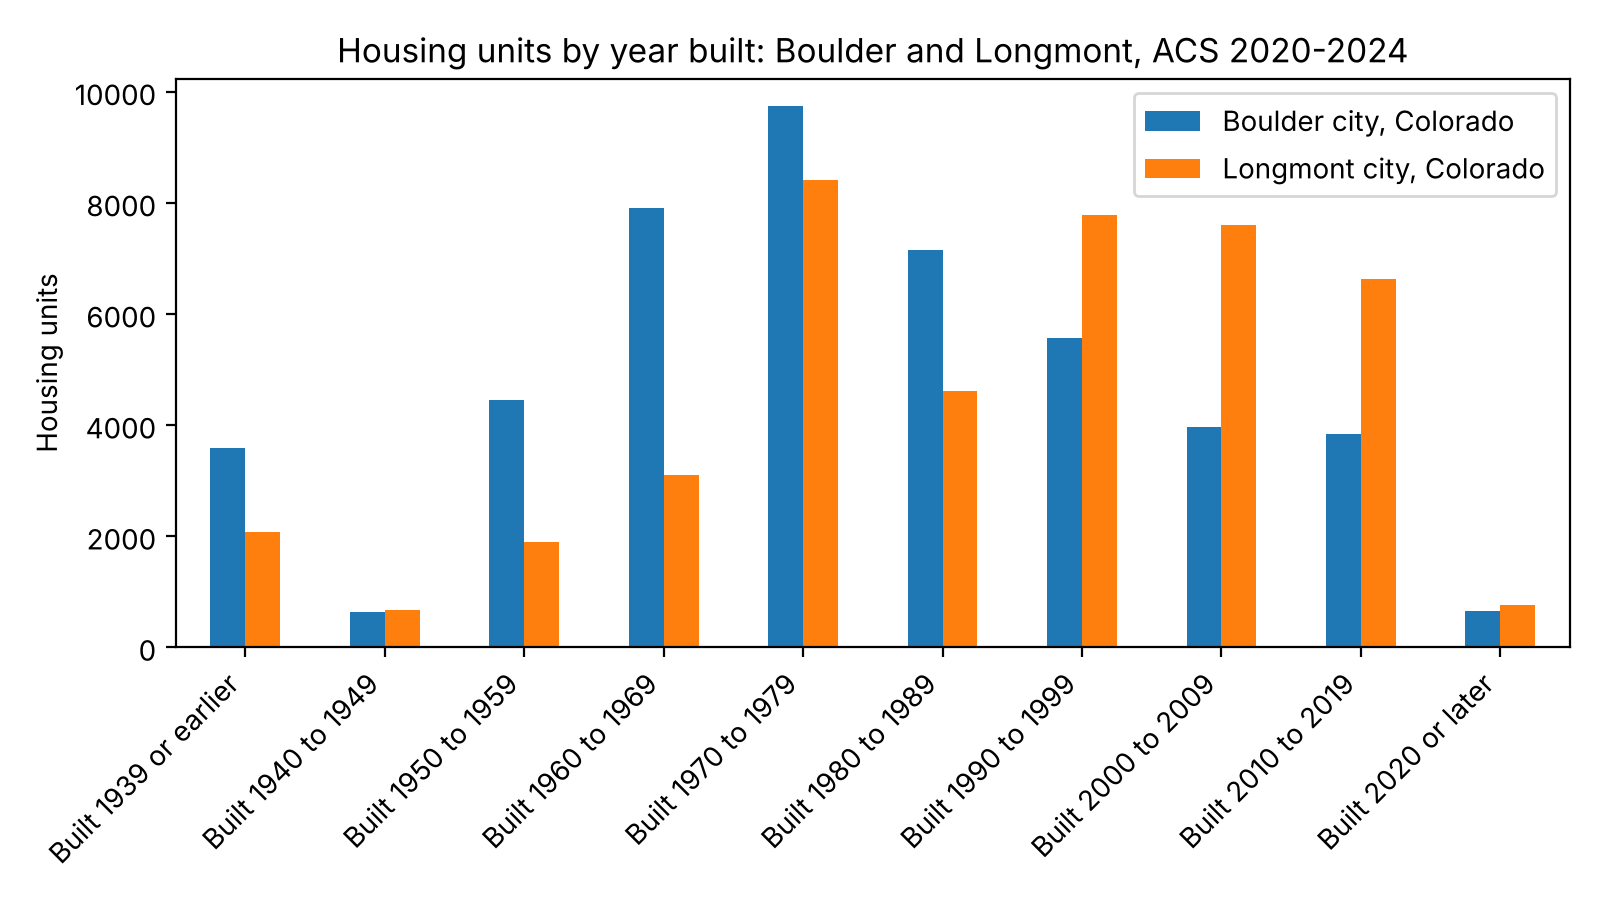
\includegraphics[width=\textwidth]{img/housing-boulder-longmont.png}\\
            {\scriptsize Drawn by the chapter's code from the Census Bureau's API, 2026-10-25 (chapter 11, figure 11.5).}

            \medskip
            \raggedright
            \textbf{Microsprint}\\[2pt]
            {\footnotesize Counts don't compare cities of different sizes; shares do. Built in 2000 or later: Castle Rock 71\%, Fort Collins 37\%, Longmont 34\%, Lakewood 18\%, Boulder 18\%.\par}
        \end{column}
    \end{columns}
\end{frame}

\begin{frame}[fragile]{Check a number against its margin}
    \begin{columns}[T]
        \begin{column}{0.56\textwidth}
            Each estimate has a margin of error, the same name ending in \texttt{M}, at 90\% confidence. Step 6 asks for both:
\begin{lstlisting}
params = {"get": "NAME,B19013_001E,B19013_001M",
          "for": "place:07850,45970",
          "in": "state:08", "key": census_key}
...
incomes["low"] = incomes["B19013_001E"] - incomes["B19013_001M"]
incomes["high"] = incomes["B19013_001E"] + incomes["B19013_001M"]
\end{lstlisting}
            \begin{center}\footnotesize
            \begin{tabular}{@{}lrrrr@{}}
                \toprule
                \textbf{City} & \textbf{Estimate} & \textbf{Margin} & \textbf{Low} & \textbf{High} \\
                \midrule
                Boulder & 87,493 & 6,221 & 81,272 & 93,714 \\
                Longmont & 90,671 & 2,975 & 87,696 & 93,646 \\
                \bottomrule
            \end{tabular}
            \end{center}
        \end{column}
        \begin{column}{0.4\textwidth}
            \begin{alertblock}{The ranges overlap}
                \footnotesize From \$87,696 to \$93,646, both are possible. The survey can't say which city's households earn more.
            \end{alertblock}
            \textbf{Discuss}\\[2pt]
            {\footnotesize Boulder's margin is twice Longmont's. What about the city could make its estimate less certain?\par}
            \medskip
            {\footnotesize Which checks like this one could a pipeline run on its own, every time it runs?\par}
        \end{column}
    \end{columns}
\end{frame}

\begin{frame}[fragile]{When there's no estimate: \texttt{-666666666}}
    \begin{columns}[T]
        \begin{column}{0.56\textwidth}
            Step 7 asks for every place in Colorado, \texttt{for=place:*} with \texttt{in=state:08}, and looks before it trusts:
\begin{lstlisting}
places["income"].describe().round()
# count          482.0
# mean    -114723934.0
# min     -666666666.0
# max         250001.0
\end{lstlisting}
            \small 83 of the 482 places have no median-income estimate: too few households answered. The API doesn't leave the value out; it sends a number that can't be an income. (250,001 is a cap: ``\$250,000 or more''.)

            \medskip
            \begin{center}\footnotesize
            \begin{tabular}{@{}lrr@{}}
                \toprule
                \textbf{Place} & \textbf{People} & \textbf{Median income} \\
                \midrule
                Boulder & 106,433 & 87,493 \\
                Campo & 58 & 53,125 ($\pm$40,478) \\
                Bonanza & 20 & \texttt{-666666666} \\
                Carbonate & 0 & \texttt{-666666666} \\
                \bottomrule
            \end{tabular}
            \end{center}
        \end{column}
        \begin{column}{0.4\textwidth}
            \begin{alertblock}{Average it as is}
                \footnotesize The mean of those four is $-333{,}298{,}178$. Mask the codes first, \texttt{towns.mask(towns < 0)}, and it's 70,309.
            \end{alertblock}
            \textbf{What the codes mean}\\[2pt]
            {\footnotesize The Census Bureau's notes on estimate and annotation values list each one; a margin of error of \texttt{-222222222} goes with it.\par}
            \medskip
            \textbf{Discuss}\\[2pt]
            {\footnotesize Carbonate has no residents, yet it has a row. What does the Census count as a place?\par}
        \end{column}
    \end{columns}
\end{frame}

\begin{frame}[fragile]{FRED: find the series, then ask what it is}
    \begin{columns}[T]
        \begin{column}{0.5\textwidth}
            Every one of FRED's 800,000 series has an \textbf{ID} (1), on its page. The \texttt{series} endpoint describes it; \texttt{series/observations} sends its values:
\begin{lstlisting}
fred_base = "https://api.stlouisfed.org/fred"
params = {"series_id": "MHICO08013A052NCEN",
          "api_key": fred_key, "file_type": "json",
          "observation_end": "2024-12-31"}
data = requests.get(f"{fred_base}/series/observations",
                    params=params, headers=HEADERS).json()
income = pd.DataFrame(data["observations"])[["date", "value"]]
income["value"] = pd.to_numeric(income["value"],
                                errors="coerce")  # "." is missing
\end{lstlisting}
            \small 2024: \$103,293 (2) --- not the Census API's \$103,994. Different programs: name the one you cite.
        \end{column}
        \begin{column}{0.46\textwidth}
            \centering
            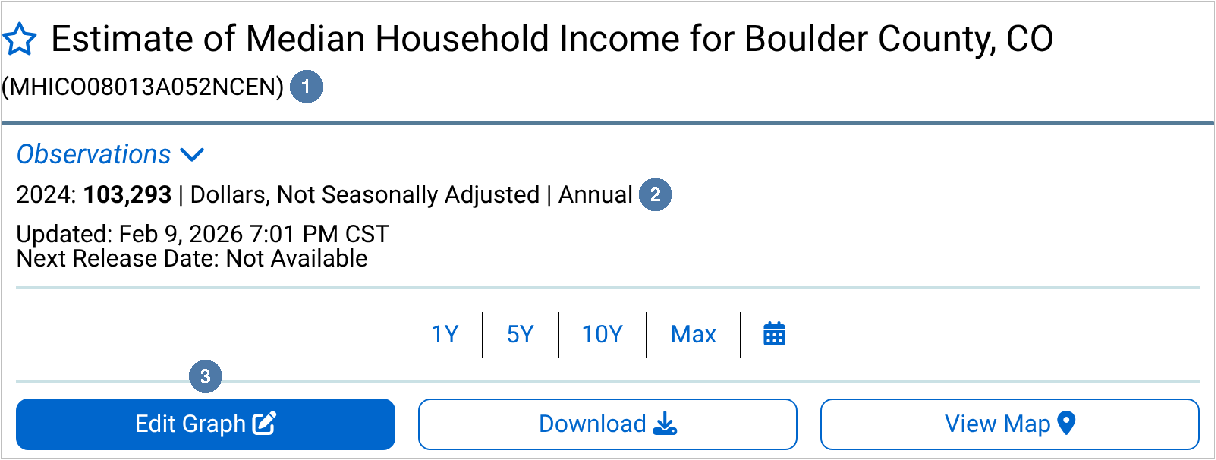
\includegraphics[width=\textwidth]{img/fred-series_annotated.pdf}\\
            {\scriptsize Boulder County's median household income on FRED, captured 2026-10-25 (chapter 11, figure 11.2).}
        \end{column}
    \end{columns}
\end{frame}

\begin{frame}[fragile]{Let the server compute: \texttt{units}}
    \begin{columns}[T]
        \begin{column}{0.56\textwidth}
            Step 9 gathers Step 8's lines into \texttt{fred\_observations(series\_id, **params)}. Then the \textit{same series} twice more, one parameter changed:
\begin{lstlisting}
change = fred_observations("MHICO08013A052NCEN",
            units="chg", observation_end="2024-12-31")
growth = fred_observations("MHICO08013A052NCEN",
            units="pch", observation_end="2024-12-31")
\end{lstlisting}
            \begin{center}\footnotesize
            \begin{tabular}{@{}rrrr@{}}
                \toprule
                \textbf{Year} & \textbf{Dollars} & \textbf{Change} & \textbf{Percent change} \\
                \midrule
                2022 & 96,584 & 6,257 & 6.9 \\
                2023 & 97,170 & 586 & 0.6 \\
                2024 & 103,293 & 6,123 & 6.3 \\
                \bottomrule
            \end{tabular}
            \end{center}
        \end{column}
        \begin{column}{0.4\textwidth}
            \textbf{What \texttt{units} can be}\\[2pt]
            {\footnotesize
            \begin{tabular}{@{}ll@{}}
                \texttt{lin} & as published \\
                \texttt{chg} & change \\
                \texttt{ch1} & change from a year before \\
                \texttt{pch} & percent change \\
                \texttt{pc1} & percent change from a year before \\
                \texttt{log} & natural logarithm \\
            \end{tabular}\par}
            \medskip
            \textbf{Microsprint}\\[2pt]
            {\footnotesize In which years did the income \textit{fall}? Six, from 2001 to 2020; the largest, \$3,003 in 2009.\par}
        \end{column}
    \end{columns}
\end{frame}

% =========================================================================
\section{Friday · Live-Coding Lab}
% =========================================================================

% The code on these frames is the lab's Part 3 (labs/week-11/lab-11-key.ipynb), rebuilt after
% Monday's class (#151) and run live on 2026-10-26, following chapter 11 at textbook 6f4cd3f.
% Figures are synced from the chapter.
\begin{frame}{Today: Part 3, more of FRED, then the EIA}
    \begin{columns}[T]
        \begin{column}{0.56\textwidth}
            \dayband{Lab}{Steps 10--15, about 35 minutes}
            \begin{itemize}\small
                \item \textbf{FRED} computes one more thing: a lower \textbf{frequency}, and inflation from it; then Denver against the nation
                \item The \textbf{EIA} (U.S. Energy Information Administration) \textbf{filters}: one state, one sector, one column, one span of years. Today's idea: \textit{let the server filter}
                \item Download the new \texttt{lab-11.ipynb}; start at \textbf{Step 10}, which sets up again
            \end{itemize}

            \medskip
            \dayband{Then}{the textbook, 15 minutes}
            \begin{itemize}\small
                \item What the lab turned up in chapter 11, as a pull request
            \end{itemize}
        \end{column}
        \begin{column}{0.4\textwidth}
            \begin{alertblock}{Two keys today}
                \footnotesize \texttt{FRED\_KEY} and \texttt{EIA\_KEY}. A \texttt{KeyError}? Wednesday's fix: \texttt{conda env config vars set}, then restart Jupyter.
            \end{alertblock}
            \textbf{No key yet?}\\[2pt]
            {\footnotesize The EIA's arrives by email within minutes. Follow along from the key until it does.\par}
            \medskip
            \textbf{In the chapter, not the lab}\\[2pt]
            {\footnotesize Congress.gov's links, paging with \texttt{offset} and \texttt{next}, and the join of the Census Bureau's incomes with the EIA's electricity bills.\par}
        \end{column}
    \end{columns}
\end{frame}

\begin{frame}[fragile]{Let the server compute: \texttt{frequency}, then \texttt{units}}
    \begin{columns}[T]
        \begin{column}{0.56\textwidth}
            One series, \texttt{CPIAUCNS} (the national Consumer Price Index, monthly), three requests:
\begin{lstlisting}
years = {"observation_start": "2015-01-01",
         "observation_end": "2025-12-31"}
monthly = fred_observations("CPIAUCNS", **years)
annual = fred_observations("CPIAUCNS", frequency="a",
            aggregation_method="avg", **years)
inflation = fred_observations("CPIAUCNS", frequency="a",
            aggregation_method="avg", units="pc1", **years)
\end{lstlisting}
            \small FRED lowers the frequency first, then applies the units: each year's mean of twelve months, then its percent change from the year before.
        \end{column}
        \begin{column}{0.4\textwidth}
            \textbf{Trust, but check once}\\[2pt]
            {\footnotesize Microsprint: the same numbers from \texttt{monthly}, with \texttt{groupby()} and \texttt{pct\_change()}.\par}
            \medskip
            {\footnotesize
            \begin{tabular}{@{}rrr@{}}
                \toprule
                \textbf{Year} & \textbf{FRED} & \textbf{pandas} \\
                \midrule
                2023 & 4.1 & 4.1 \\
                2024 & 2.9 & 2.9 \\
                2025 & 2.6 & 2.6 \\
                \bottomrule
            \end{tabular}\par}
            \medskip
            {\footnotesize Why can FRED give 2015's inflation, and pandas can't?\par}
        \end{column}
    \end{columns}
\end{frame}

\begin{frame}[fragile]{Denver against the nation}
    \begin{columns}[T]
        \begin{column}{0.36\textwidth}
            The Bureau of Labor Statistics' CPI for the Denver area, \texttt{CUUSA433SA0}, is annual already: it needs only \texttt{units="pc1"}.
\begin{lstlisting}
denver = fred_observations(
    "CUUSA433SA0", units="pc1", **years)
cpi = denver.merge(inflation, on="date",
    suffixes=("_denver", "_national"))
\end{lstlisting}
            \small Denver ran ahead from 2015 to 2020, and behind since 2024. Housing is the largest part of the CPI: what would you ask FRED next?
        \end{column}
        \begin{column}{0.6\textwidth}
            \centering
            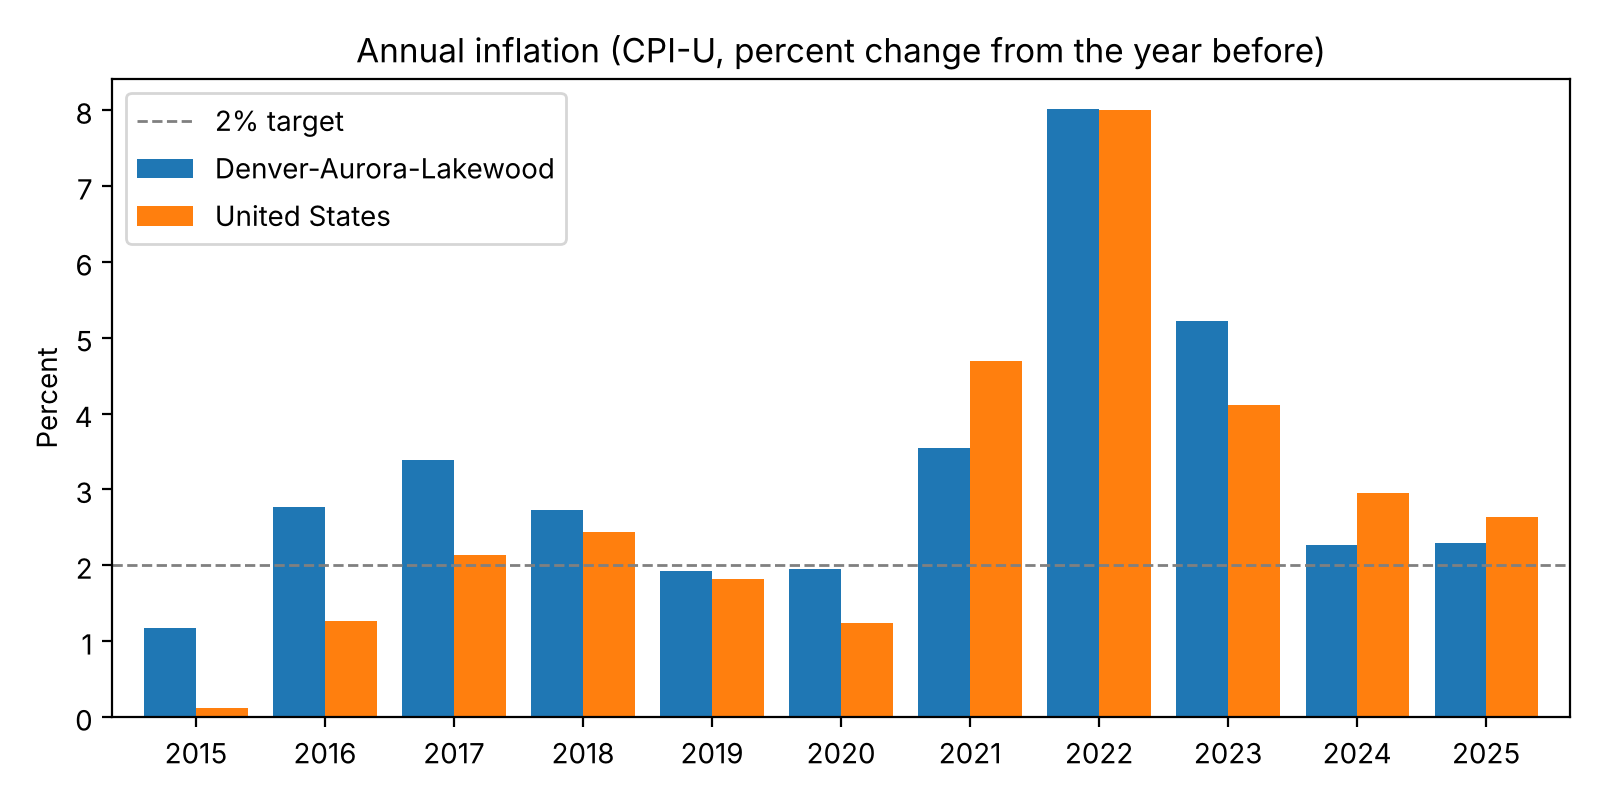
\includegraphics[width=\textwidth]{img/cpi-denver-national.png}\\
            {\scriptsize Drawn by the chapter's code from FRED, 2026-10-25 (chapter 11, figure 11.6). The dashed line is the Federal Reserve's 2\% target.}
        \end{column}
    \end{columns}
\end{frame}

\begin{frame}[fragile]{EIA: routes that describe themselves}
    \begin{columns}[T]
        \begin{column}{0.54\textwidth}
            The EIA's API is a tree of \textbf{routes}. Ask for one without \texttt{data/}, and it says what it holds:
\begin{lstlisting}
eia_base = "https://api.eia.gov/v2"
meta = requests.get(f"{eia_base}/electricity/retail-sales/",
                    params={"api_key": eia_key},
                    headers=HEADERS).json()["response"]
print([f["id"] for f in meta["facets"]])
# ['stateid', 'sectorid']
for column, about in meta["data"].items():
    print(column, "|", about["units"])
# price | cents per kilowatt-hour   ...and 3 more
\end{lstlisting}
            \small A \textbf{facet} filters the rows; a \textbf{data column} (1) is what each row holds. Monday's idea, \textit{what can I ask for?}, from a different API: here the route describes itself, where the Census Bureau's catalog was \texttt{groups.json}.
        \end{column}
        \begin{column}{0.42\textwidth}
            \centering
            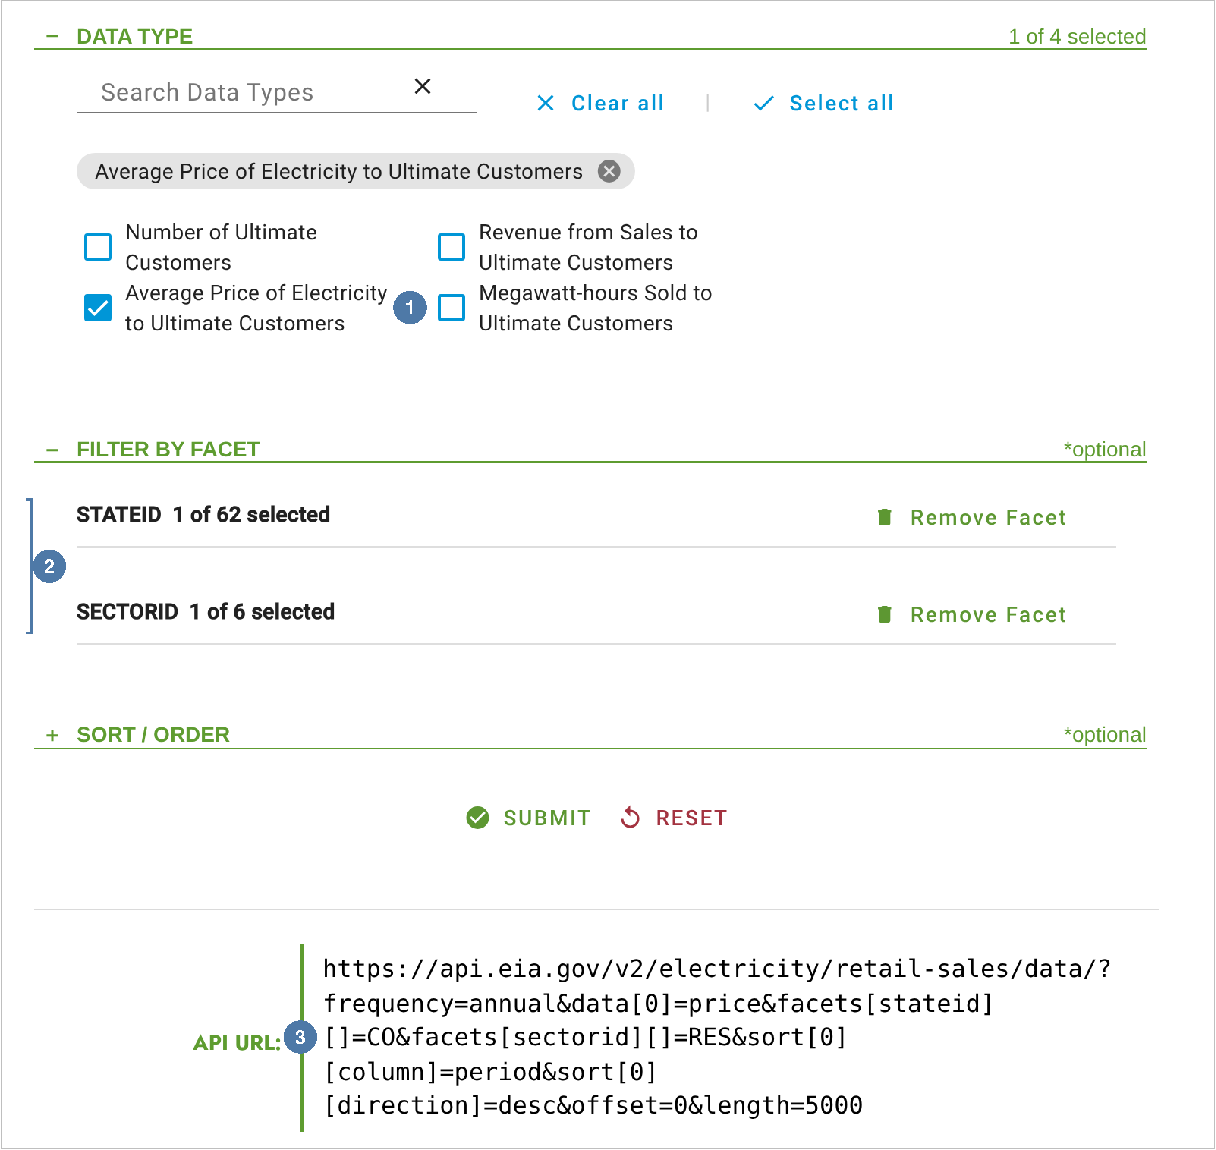
\includegraphics[width=0.92\textwidth]{img/eia-browser_annotated.pdf}\\
            {\scriptsize The EIA's API Dashboard, captured 2026-10-25 (chapter 11, figure 11.3): its menus (2) are those routes, and it writes the request (3).}
        \end{column}
    \end{columns}
\end{frame}

\begin{frame}[fragile]{Let the server filter}
    \begin{columns}[T]
        \begin{column}{0.56\textwidth}
            Add \texttt{data/} to the route, and each parameter narrows the rows. The brackets are part of the names:
\begin{lstlisting}
params = {"frequency": "annual", "data[]": "price",
          "facets[stateid][]": "CO",
          "facets[sectorid][]": "RES",   # homes
          "start": "2001", "end": "2025",
          "sort[0][column]": "period",
          "sort[0][direction]": "asc",
          "api_key": eia_key}
prices = requests.get(f"{eia_base}/electricity/retail-sales/data/",
            params=params, headers=HEADERS).json()["response"]
print("Rows:", prices["total"])   # Rows: 25
\end{lstlisting}
            \small 25 rows, from a route that holds every state and sector by month, quarter, and year. Colorado's homes paid 15.69 cents a kilowatt-hour in 2025.
        \end{column}
        \begin{column}{0.4\textwidth}
            \textbf{Microsprint}\\[2pt]
            {\footnotesize Change one facet: a sector (\texttt{COM}, \texttt{IND}) or a state (\texttt{UT}, \texttt{NM}). Colorado's businesses paid 12.37 cents in 2025.\par}
            \medskip
            \textbf{Still strings}\\[2pt]
            {\footnotesize Prices and \texttt{total} arrive as text, like the Census Bureau's numbers: \texttt{pd.to\_numeric()} before any math.\par}
            \medskip
            \textbf{Filter before you page}\\[2pt]
            {\footnotesize The EIA sends at most 5,000 rows a request. A facet, a shorter span, or a lower frequency may fit the answer in one; the chapter's ``Paging with \texttt{offset} and \texttt{length}'' covers the rest.\par}
        \end{column}
    \end{columns}
\end{frame}

\begin{frame}{What a filtered request can show}
    \begin{columns}[T]
        \begin{column}{0.36\textwidth}
            The chapter asks the same API for Colorado's annual generation from five sources, plus the total: one facet, six values, one request.

            \medskip
            \small Coal made 76.7\% of the state's electricity in 2001 and 24.7\% in 2025. Wind grew from almost nothing to 30.0\%; 2024 was the first year coal wasn't the largest source.
        \end{column}
        \begin{column}{0.6\textwidth}
            \centering
            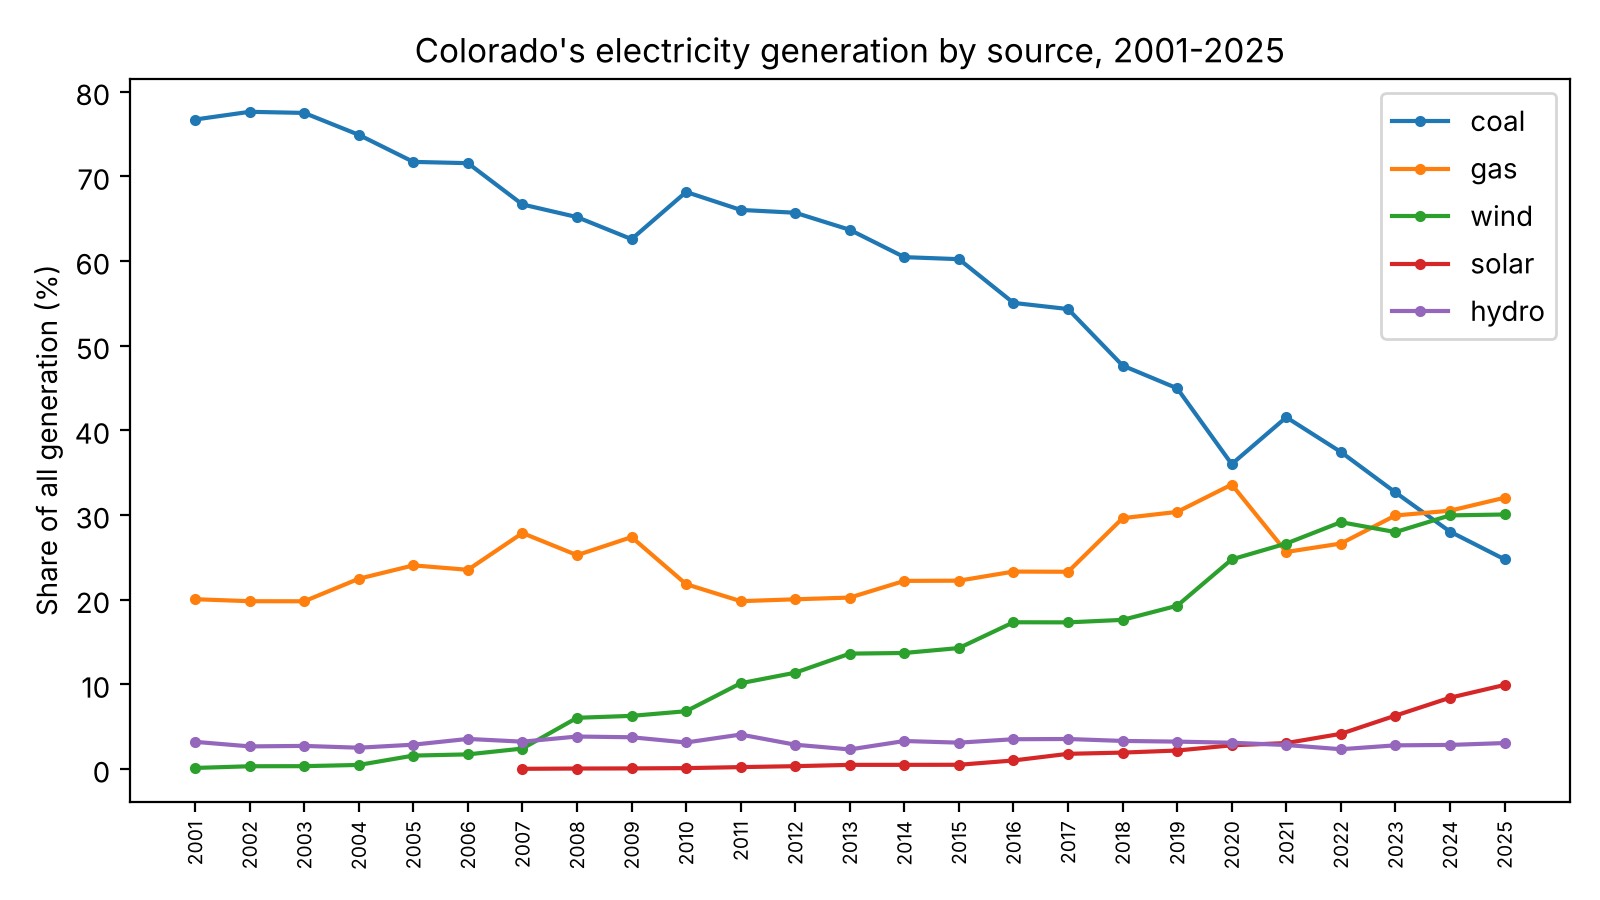
\includegraphics[width=\textwidth]{img/co-generation-mix.png}\\
            {\scriptsize Drawn by the chapter's code from the EIA's API, 2026-10-25 (chapter 11, figure 11.7).}
        \end{column}
    \end{columns}
\end{frame}

\begin{frame}{Friday: from the lab to the textbook (15 minutes)}
    \begin{columns}[T]
        \begin{column}{0.58\textwidth}
            Look back at what the lab turned up in chapter 11, and propose one change as a \textbf{pull request}:
            \begin{itemize}\small
                \item \textbf{A cell that broke.} On Monday, \texttt{os.environ["CENSUS\_KEY"]} stopped with a \texttt{KeyError} for some of us after \texttt{export}. Does ``Setting Environment Variables'' say why, and what to do?
                \item \textbf{A sentence that confused.} Which step needed the website beside the API to make sense? Does the chapter's tour do that for the Census table, and could it do more?
                \item \textbf{An output that has changed.} The EIA's 2025 figures are preliminary. Compare Step 14's prices with the chapter's.
                \item \textbf{A microsprint that would make a good exercise.} Searching \texttt{groups.json} for your own topic (Step 1), or two cities' margins (Step 6).
            \end{itemize}
        \end{column}
        \begin{column}{0.38\textwidth}
            \textbf{How to propose one}\\[2pt]
            {\footnotesize The course's \texttt{handouts/common/revision-framework.md} says what each kind of change needs to be accepted.\par}
            \medskip
            \textbf{A good review}\\[2pt]
            {\footnotesize Run the change; name the line; separate ``must fix'' from ``nice to have''; end with a verdict.\par}
            \medskip
        \end{column}
    \end{columns}
\end{frame}

% =========================================================================
\begin{frame}{Key takeaways}
    \begin{enumerate}
        \item Government APIs serve \textbf{public mandates}: the census, the Federal Reserve's data, the EIA's statistics.
        \item Each carried one idea you'll meet again: \textbf{ask what you can ask for} (Census), \textbf{let the server compute} (FRED), \textbf{let the server filter} (EIA).
        \item \textbf{Start from the website}: find the number there, then ask the API for the same number, and check that they match.
        \item \textbf{Read what isn't a number}: a margin of error, a code like \texttt{-666666666}, a cap at \$250,000, a \texttt{"."} for missing.
        \item \textbf{Keys stay out of notebooks}: environment variables, checked with \texttt{set} or \texttt{MISSING}, never printed.
    \end{enumerate}
\end{frame}

\end{document}
